% Options for packages loaded elsewhere
% Options for packages loaded elsewhere
\PassOptionsToPackage{unicode}{hyperref}
\PassOptionsToPackage{hyphens}{url}
\PassOptionsToPackage{dvipsnames,svgnames,x11names}{xcolor}
%
\documentclass[
  british,
  12pt,
  a4paper,
]{report}
\usepackage{xcolor}
\usepackage[top=30mm,left=30mm,right=30mm,bottom=30mm]{geometry}
\usepackage{amsmath,amssymb}
\setcounter{secnumdepth}{5}
\usepackage{iftex}
\ifPDFTeX
  \usepackage[T1]{fontenc}
  \usepackage[utf8]{inputenc}
  \usepackage{textcomp} % provide euro and other symbols
\else % if luatex or xetex
  \usepackage{unicode-math} % this also loads fontspec
  \defaultfontfeatures{Scale=MatchLowercase}
  \defaultfontfeatures[\rmfamily]{Ligatures=TeX,Scale=1}
\fi
\usepackage{lmodern}
\ifPDFTeX\else
  % xetex/luatex font selection
\fi
% Use upquote if available, for straight quotes in verbatim environments
\IfFileExists{upquote.sty}{\usepackage{upquote}}{}
\IfFileExists{microtype.sty}{% use microtype if available
  \usepackage[]{microtype}
  \UseMicrotypeSet[protrusion]{basicmath} % disable protrusion for tt fonts
}{}
\usepackage{setspace}
\makeatletter
\@ifundefined{KOMAClassName}{% if non-KOMA class
  \IfFileExists{parskip.sty}{%
    \usepackage{parskip}
  }{% else
    \setlength{\parindent}{0pt}
    \setlength{\parskip}{6pt plus 2pt minus 1pt}}
}{% if KOMA class
  \KOMAoptions{parskip=half}}
\makeatother
% Make \paragraph and \subparagraph free-standing
\makeatletter
\ifx\paragraph\undefined\else
  \let\oldparagraph\paragraph
  \renewcommand{\paragraph}{
    \@ifstar
      \xxxParagraphStar
      \xxxParagraphNoStar
  }
  \newcommand{\xxxParagraphStar}[1]{\oldparagraph*{#1}\mbox{}}
  \newcommand{\xxxParagraphNoStar}[1]{\oldparagraph{#1}\mbox{}}
\fi
\ifx\subparagraph\undefined\else
  \let\oldsubparagraph\subparagraph
  \renewcommand{\subparagraph}{
    \@ifstar
      \xxxSubParagraphStar
      \xxxSubParagraphNoStar
  }
  \newcommand{\xxxSubParagraphStar}[1]{\oldsubparagraph*{#1}\mbox{}}
  \newcommand{\xxxSubParagraphNoStar}[1]{\oldsubparagraph{#1}\mbox{}}
\fi
\makeatother


\usepackage{longtable,booktabs,array}
\usepackage{calc} % for calculating minipage widths
% Correct order of tables after \paragraph or \subparagraph
\usepackage{etoolbox}
\makeatletter
\patchcmd\longtable{\par}{\if@noskipsec\mbox{}\fi\par}{}{}
\makeatother
% Allow footnotes in longtable head/foot
\IfFileExists{footnotehyper.sty}{\usepackage{footnotehyper}}{\usepackage{footnote}}
\makesavenoteenv{longtable}
\usepackage{graphicx}
\makeatletter
\newsavebox\pandoc@box
\newcommand*\pandocbounded[1]{% scales image to fit in text height/width
  \sbox\pandoc@box{#1}%
  \Gscale@div\@tempa{\textheight}{\dimexpr\ht\pandoc@box+\dp\pandoc@box\relax}%
  \Gscale@div\@tempb{\linewidth}{\wd\pandoc@box}%
  \ifdim\@tempb\p@<\@tempa\p@\let\@tempa\@tempb\fi% select the smaller of both
  \ifdim\@tempa\p@<\p@\scalebox{\@tempa}{\usebox\pandoc@box}%
  \else\usebox{\pandoc@box}%
  \fi%
}
% Set default figure placement to htbp
\def\fps@figure{htbp}
\makeatother



\ifLuaTeX
\usepackage[bidi=basic]{babel}
\else
\usepackage[bidi=default]{babel}
\fi
% get rid of language-specific shorthands (see #6817):
\let\LanguageShortHands\languageshorthands
\def\languageshorthands#1{}
\ifLuaTeX
  \usepackage[english]{selnolig} % disable illegal ligatures
\fi


\setlength{\emergencystretch}{3em} % prevent overfull lines

\providecommand{\tightlist}{%
  \setlength{\itemsep}{0pt}\setlength{\parskip}{0pt}}



 


% LaTeX preamble for thesis PDF
\usepackage{graphicx}
\usepackage[T1]{fontenc}
\usepackage[sc]{mathpazo}   % Palatino with small caps and old-style figures — thin, fine strokes
\linespread{1.05}           % Palatino needs slightly more leading




\usepackage{xcolor}
\usepackage{hyperref}
\hypersetup{colorlinks=true,linkcolor=black,urlcolor=blue,citecolor=black}
\usepackage{setspace}
\onehalfspacing
\usepackage{booktabs}
\usepackage{longtable}
\usepackage{enumitem}
\usepackage{amsmath}
\usepackage{amssymb}

% Define horizontal rule command for title page
\newcommand{\HRule}{\rule{\linewidth}{0.5mm}}


% Remove the automatic "Chapter X" heading at the top of each chapter page
\usepackage{titlesec}
\titleformat{\chapter}[block]{\normalfont\huge\bfseries}{}{0pt}{}
\titlespacing*{\chapter}{0pt}{0pt}{20pt}
\makeatletter
\@ifpackageloaded{bookmark}{}{\usepackage{bookmark}}
\makeatother
\makeatletter
\@ifpackageloaded{caption}{}{\usepackage{caption}}
\AtBeginDocument{%
\ifdefined\contentsname
  \renewcommand*\contentsname{Table of contents}
\else
  \newcommand\contentsname{Table of contents}
\fi
\ifdefined\listfigurename
  \renewcommand*\listfigurename{List of Figures}
\else
  \newcommand\listfigurename{List of Figures}
\fi
\ifdefined\listtablename
  \renewcommand*\listtablename{List of Tables}
\else
  \newcommand\listtablename{List of Tables}
\fi
\ifdefined\figurename
  \renewcommand*\figurename{Figure}
\else
  \newcommand\figurename{Figure}
\fi
\ifdefined\tablename
  \renewcommand*\tablename{Table}
\else
  \newcommand\tablename{Table}
\fi
}
\@ifpackageloaded{float}{}{\usepackage{float}}
\floatstyle{ruled}
\@ifundefined{c@chapter}{\newfloat{codelisting}{h}{lop}}{\newfloat{codelisting}{h}{lop}[chapter]}
\floatname{codelisting}{Listing}
\newcommand*\listoflistings{\listof{codelisting}{List of Listings}}
\makeatother
\makeatletter
\makeatother
\makeatletter
\@ifpackageloaded{caption}{}{\usepackage{caption}}
\@ifpackageloaded{subcaption}{}{\usepackage{subcaption}}
\makeatother
\usepackage{bookmark}
\IfFileExists{xurl.sty}{\usepackage{xurl}}{} % add URL line breaks if available
\urlstyle{same}
\hypersetup{
  pdftitle={Measuring Technical Debt in Mission Critical Trading Systems},
  pdfauthor={Tobias Zeier},
  pdflang={en-GB},
  colorlinks=true,
  linkcolor={blue},
  filecolor={Maroon},
  citecolor={Blue},
  urlcolor={Blue},
  pdfcreator={LaTeX via pandoc}}


\title{Measuring Technical Debt in Mission Critical Trading Systems}
\usepackage{etoolbox}
\makeatletter
\providecommand{\subtitle}[1]{% add subtitle to \maketitle
  \apptocmd{\@title}{\par {\large #1 \par}}{}{}
}
\makeatother
\subtitle{A Service Level Quantitative Framework}
\author{Tobias Zeier}
\date{10 August 2026}
\begin{document}
% Custom title page template for Quarto book PDF


\begin{titlepage}
% Switch to Palatino for title page only
{\fontfamily{ppl}\selectfont
\centering

% University name at the very top
{\large\textbf{{\Large U}NIVERSITY OF ESSEX ONLINE}}\\[1.2cm]

% Degree type
{\normalsize\textbf{{\large M}ASTER'S THESIS}}\\[1.6cm]

% Horizontal rule before title
\noindent\rule{\textwidth}{0.8pt}\\[0.5cm]

% Thesis title
{\LARGE\bfseries Measuring Technical Debt in Mission Critical Trading
Systems}\\[0.4cm]
{\large\bfseries A Service Level Quantitative Framework}\\[0.5cm]

% Horizontal rule after title
\noindent\rule{\textwidth}{0.8pt}\\[2.2cm]

% Author (left) and Supervisors (right) side by side
\begin{minipage}[t]{0.48\textwidth}
\raggedright
\normalsize
\textit{Author}\\
Tobias Zeier
\end{minipage}
\hfill
\begin{minipage}[t]{0.48\textwidth}
\raggedleft
\normalsize
\textit{Supervisor}\\
Dr Zahid Ullah\\[0.3cm]
\textit{Co-Supervisor}\\
Doug Millward
\end{minipage}

\vfill

% Department
{\normalsize Computing Department}\\[0.8cm]

% University logo (smaller)
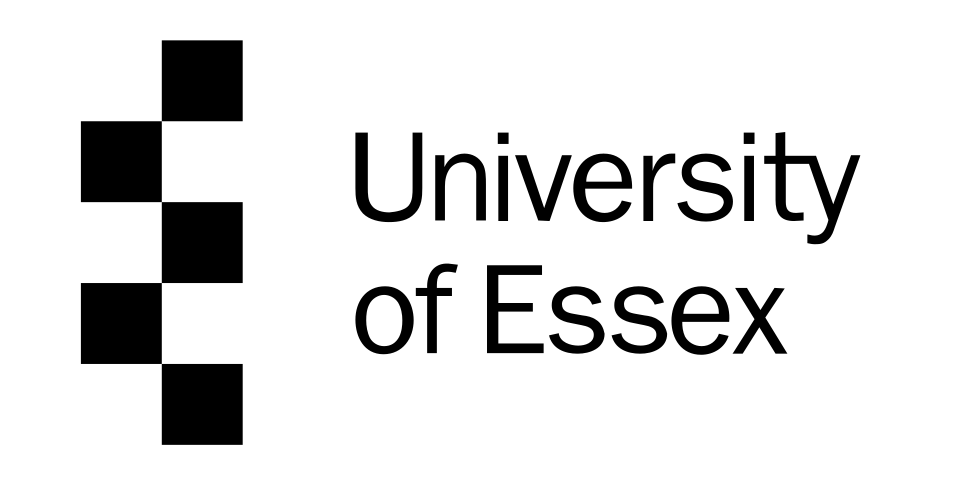
\includegraphics[width=0.22\textwidth]{university-logo.png}\\[0.7cm]

% Date at the very bottom
{\normalsize 10 August 2026}

} % end Palatino scope
\end{titlepage}

% Revert to Times New Roman for the rest of the document
{\fontfamily{ptm}\selectfont}
\cleardoublepage
\renewcommand*\contentsname{Table of contents}
{
\hypersetup{linkcolor=}
\setcounter{tocdepth}{2}
\tableofcontents
}

\setstretch{1.5}
\bookmarksetup{startatroot}

\chapter{Measuring Technical Debt in Mission Critical Trading
Systems}\label{measuring-technical-debt-in-mission-critical-trading-systems}

A Service Level Quantitative Framework

\hfill\break

\newpage

\section{Preface}\label{preface}

(Write a short preface / declaration / abstract here, or leave this
section empty for now.)

\bookmarksetup{startatroot}

\chapter{Chapters}\label{chapters}

\bookmarksetup{startatroot}

\chapter{Introduction}\label{introduction}

Start your thesis here.

\bookmarksetup{startatroot}

\chapter{Background}\label{background}

Add background on technical debt and mission-critical trading systems.

\bookmarksetup{startatroot}

\chapter{Methodology}\label{methodology}

Describe your service-level quantitative framework.

\bookmarksetup{startatroot}

\chapter{Results}\label{results}

Present your measurements and findings.

\bookmarksetup{startatroot}

\chapter{Discussion}\label{discussion}

Interpret results and implications.

\bookmarksetup{startatroot}

\chapter{Conclusion}\label{conclusion}

Summarise contributions and future work.




\end{document}
